\subsection{Reverberation recordings in the elevator}

\begin{figure}
\center{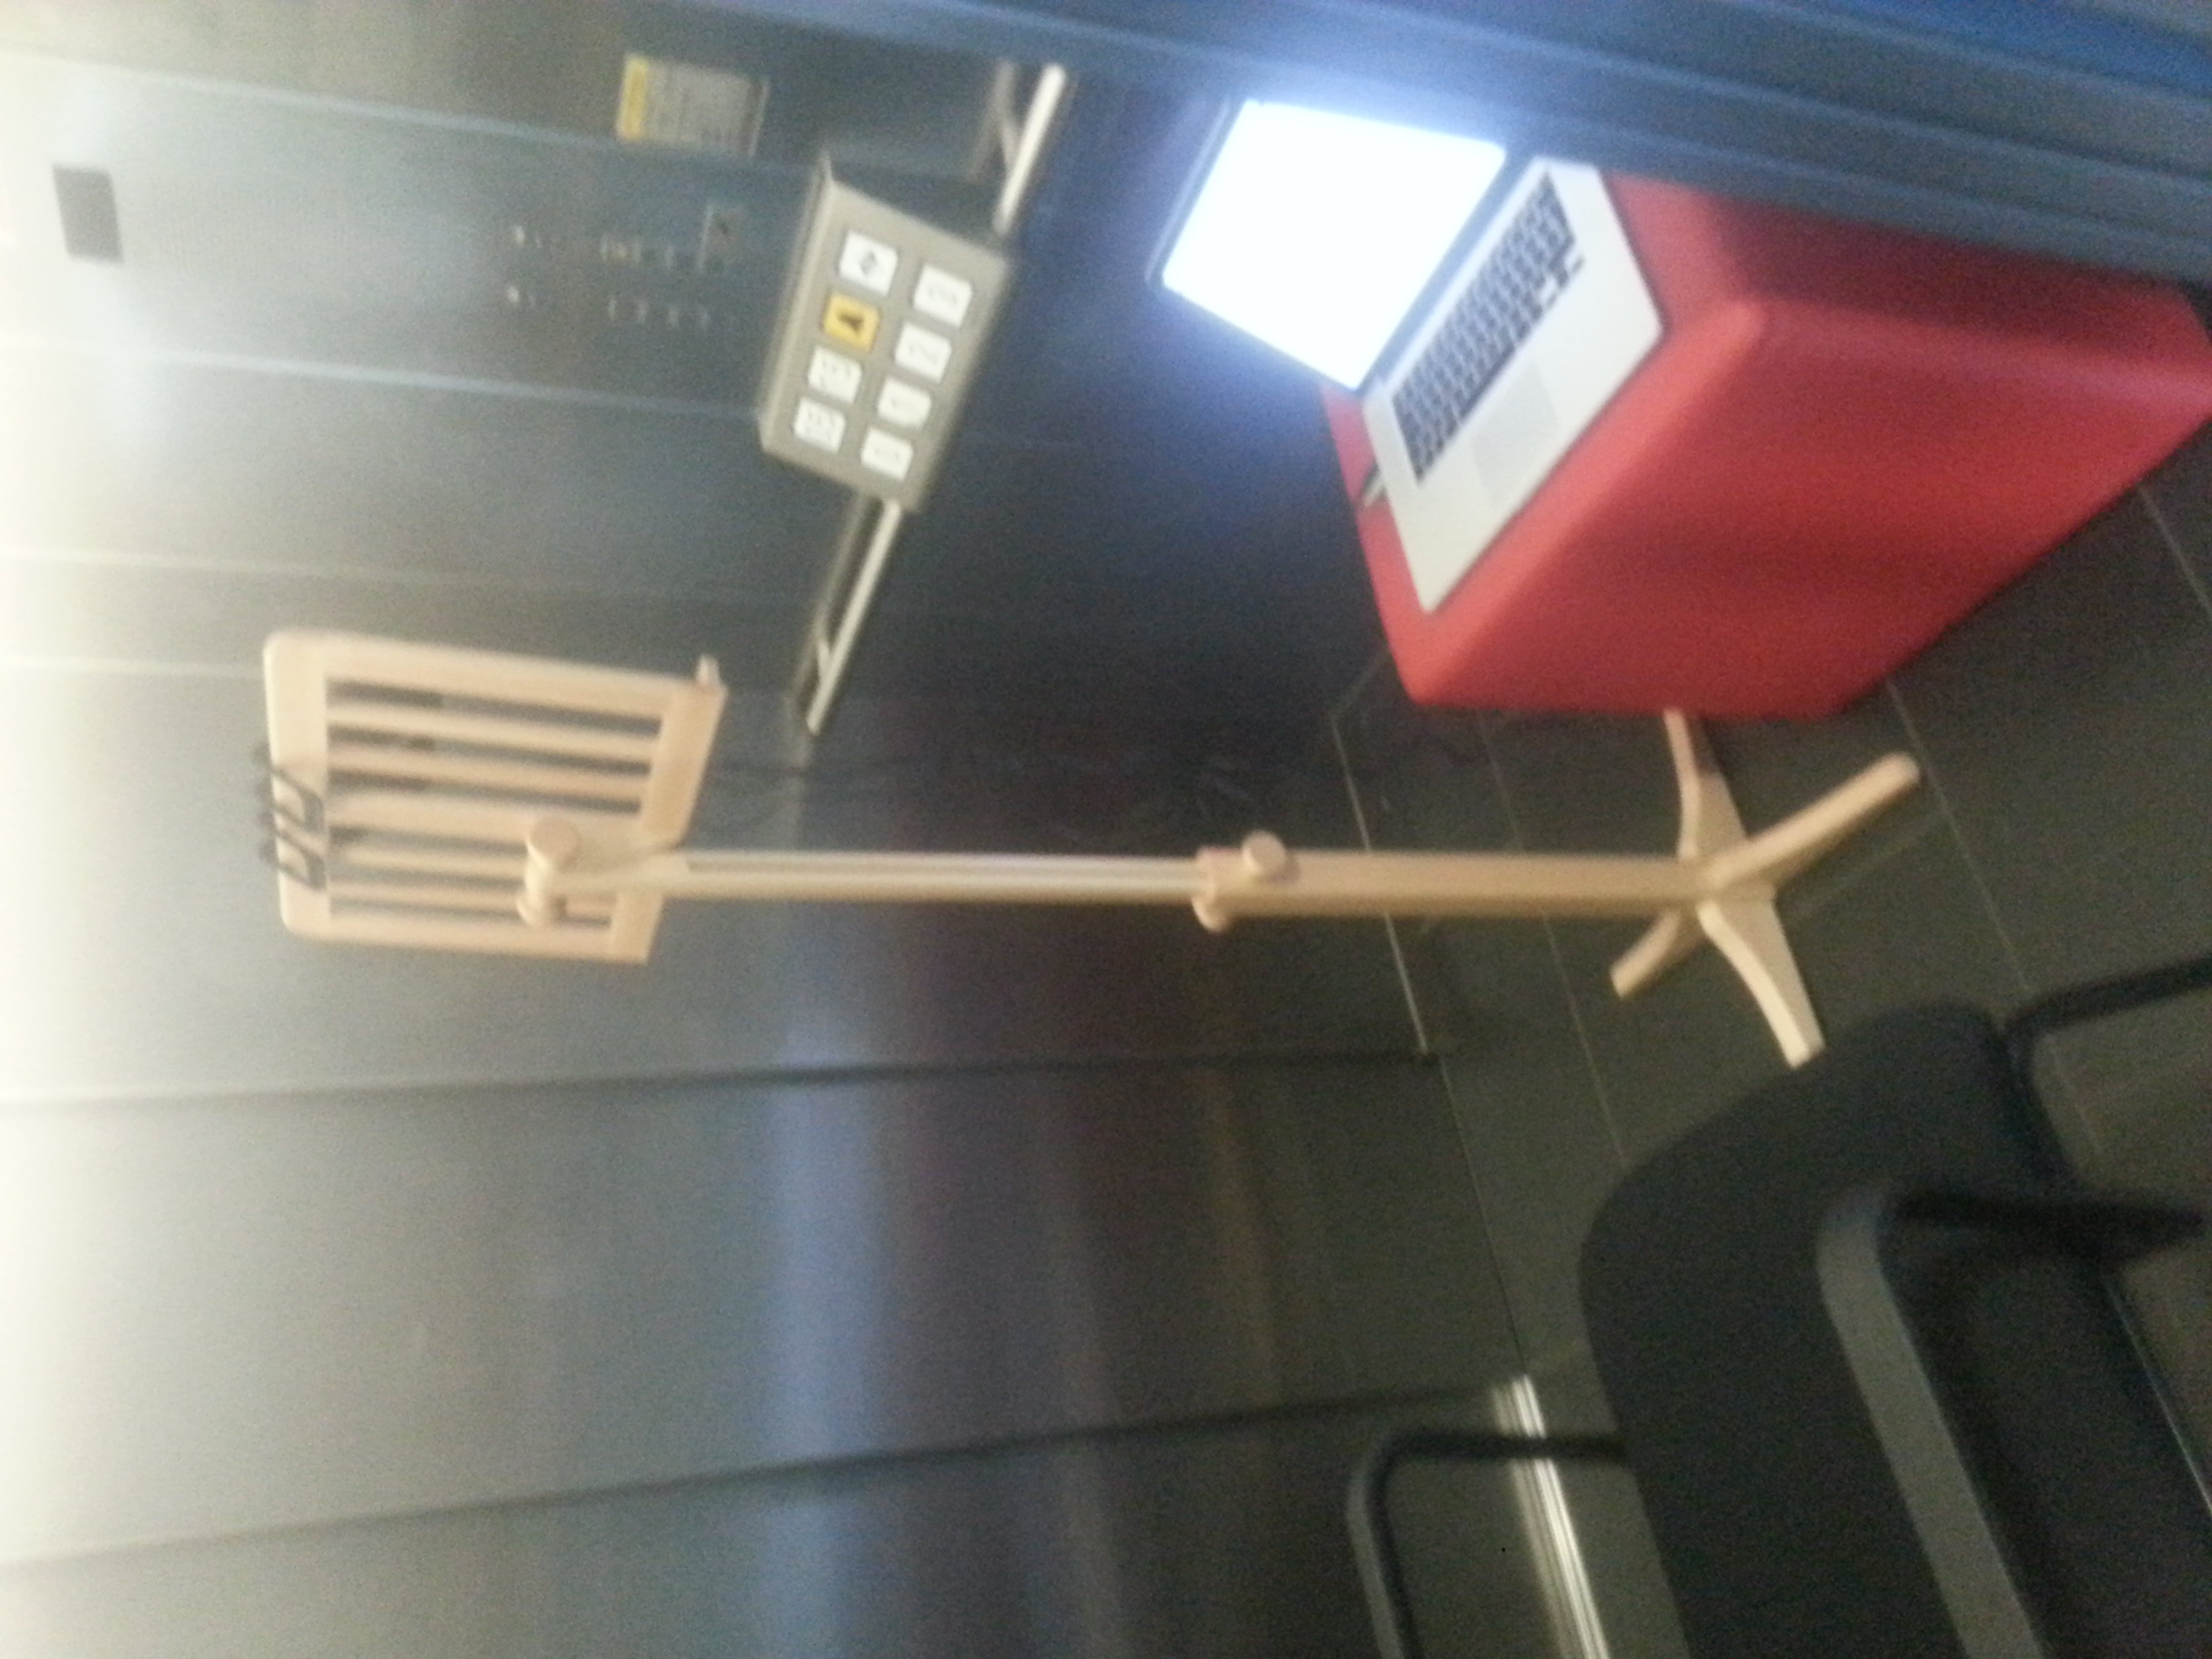
\includegraphics[scale=0.10, angle=-90]{setup_reverberation_rec.jpg}}
\caption{Recordings setup.}
\label{fig:recordingsetup}
\end{figure}


To train the accoustic model for the elevator, recordings of elevator-specific commands and phonetically balanced sentences in both English and German were made. 
Lists one and two  of the Harvard sentences\footnote{http://www.cs.columbia.edu/~hgs/audio/harvard.html} were used as phonetically balanced sentences in English and twenty sentences taken from BITS\footnote{http://www.bas.uni-muenchen.de/forschung/Bas/BasBITSUSTABLE} were used for German. 
The full list of sentences which have been used can be found in the appendix. %appendix Sätze
The sentences were read by all of the participants and recorded in a soundproof studio
This resulted in recordings of English material spoken by non-natives and German material spoken by natives and by non-natives.


To account for the noise of the elevator, its sound when moving, the sound of the doors opening and closing and the reverberation with open doors on the different floors and other noises from outside of the elevator, further recordings were made via the elevator's built-in microphone. 
The setup used for this can be seen in picture \ref{fig:recordingsetup}.
It consisted of two loudspeakers positioned on a music stand at the height of approximately 150cm, at a distance of approximately 20cm from the elevator's microphone. 
The recordings made in the lab were played through the loudspeakers and recorded with Praat via the elevator's microphone. 
While the recordings were being played, the elevator was moved between the floors, its doors were opened and closed and kept stationary with its doors opened and closed on different floors.

